\null\newpage
\clearpage

\section{Anexo}

\subsection{Diseño final - imágenes}
\begin{figure}[htb]
    \centering
    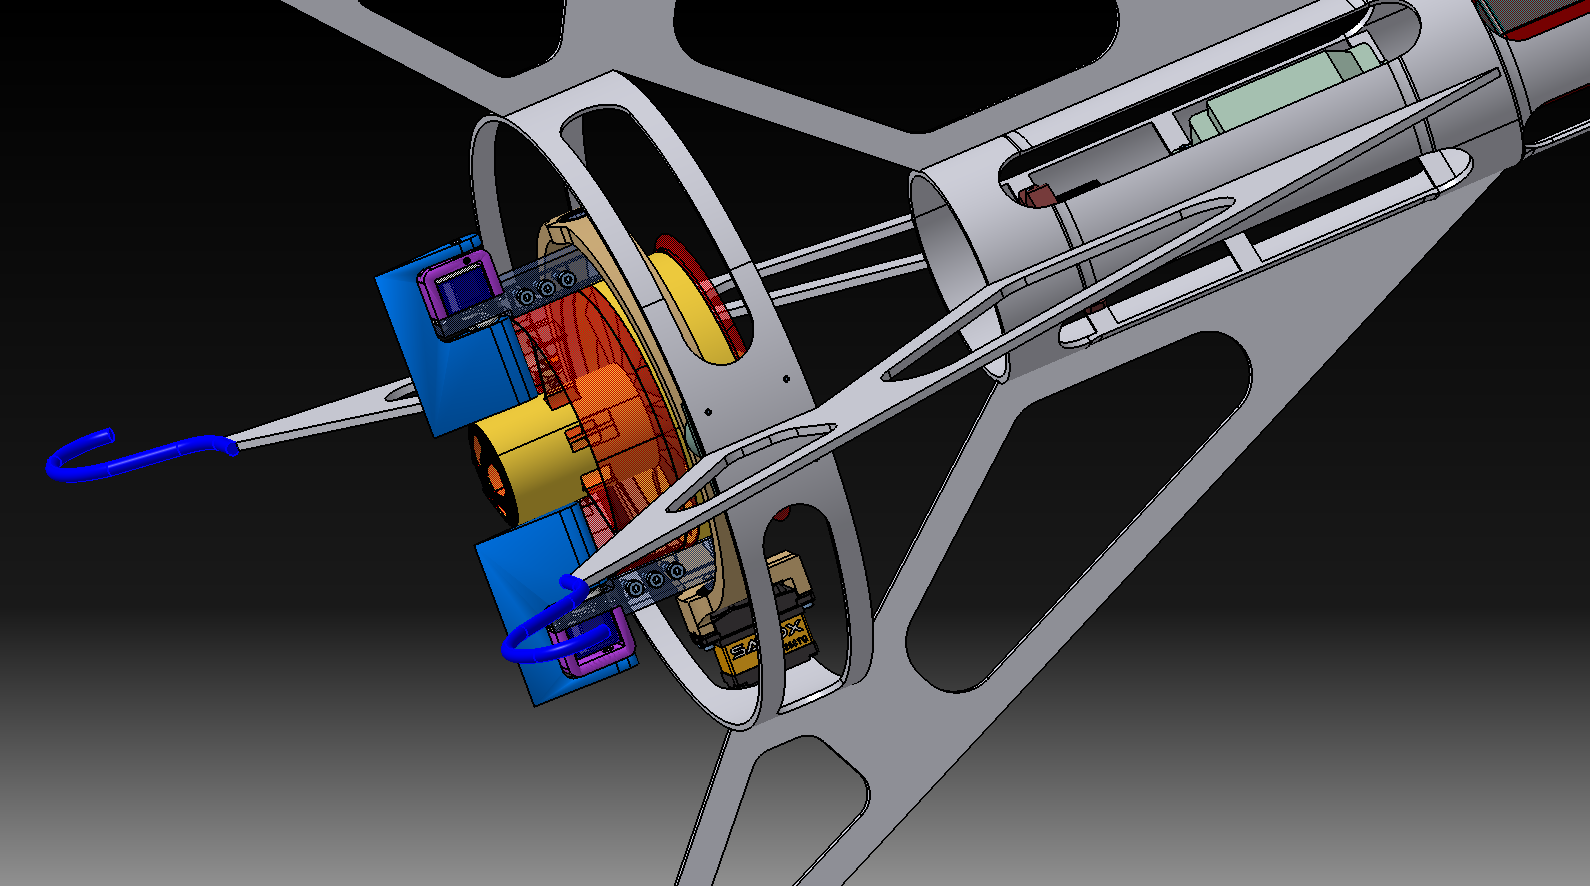
\includegraphics[width=\linewidth]{fig/design/v6_3}
    \caption{Prototipo final detalle EDF.}
    \label{fig:design/v6_3}
\end{figure}

\begin{figure}[htb]
    \centering
    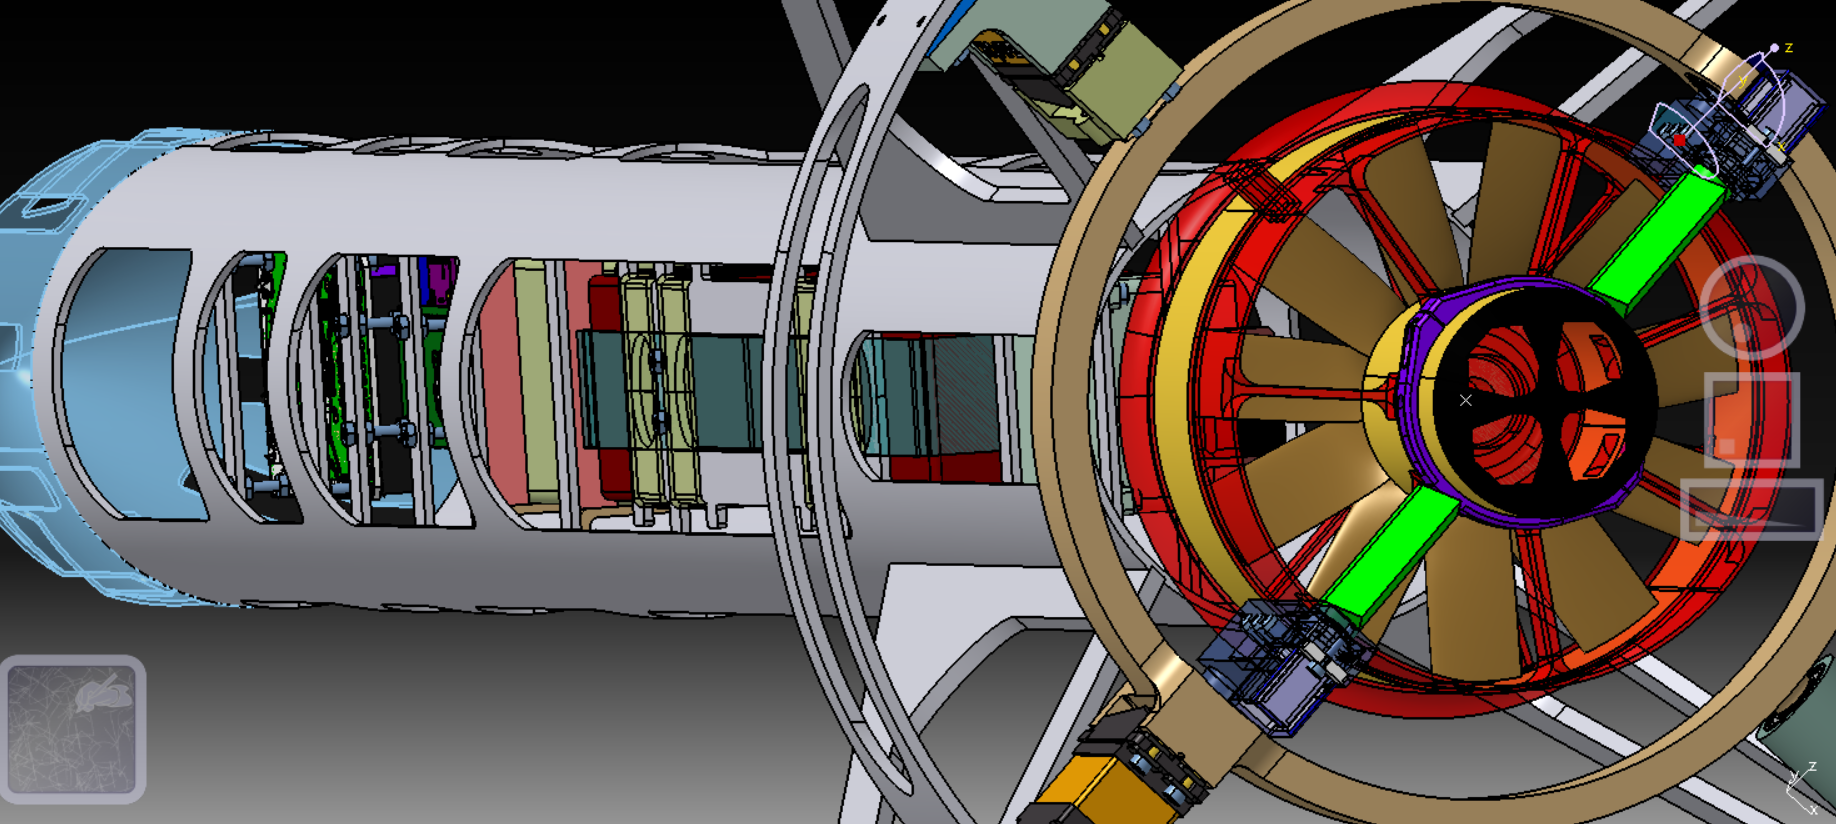
\includegraphics[width=\linewidth]{fig/design/v6_5}
    \caption{Prototipo final vista inferior detalle constructivo.}
    \label{fig:design/v6_5}
\end{figure}

\subsection{Diseños preliminares - imágenes}

\begin{figure}[htb]
    \centering
    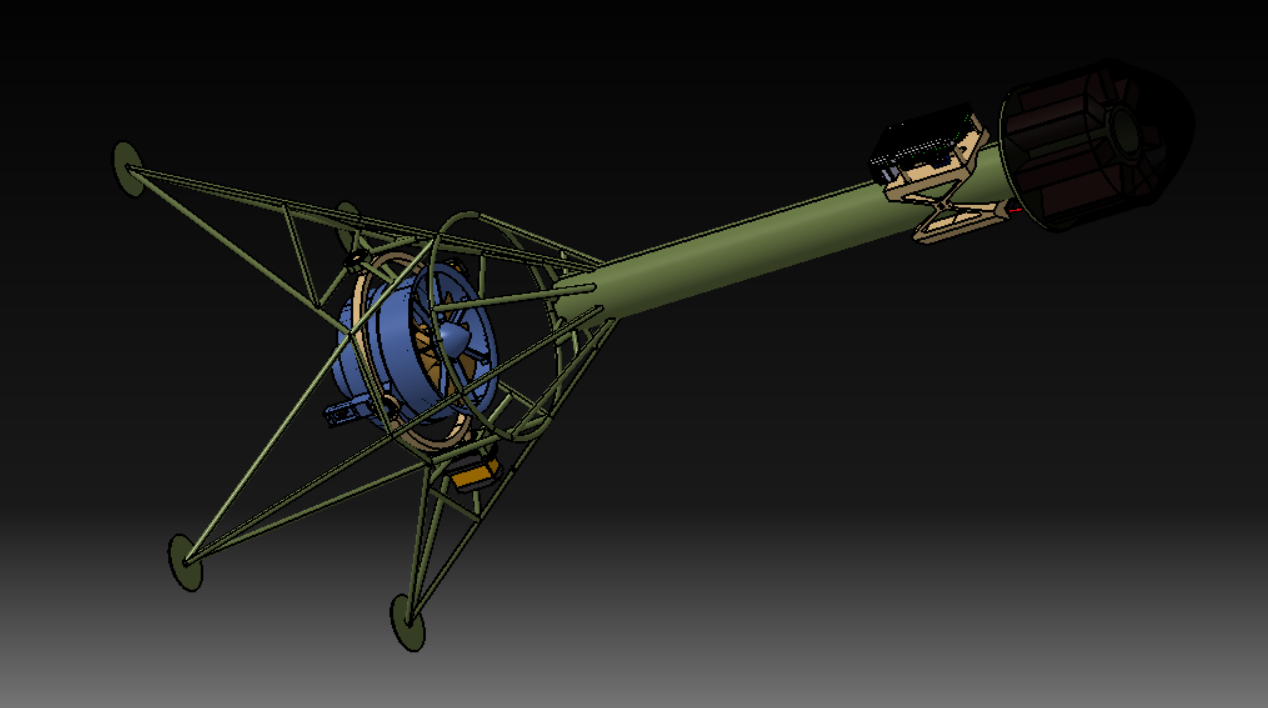
\includegraphics[width=\linewidth]{fig/design/0}
    \caption{Prototipo de fuselaje con patas reticuladas integro en aluminio, baterías en la nariz, aviónica debajo de la nariz, sin sistema anti rolido.}
    \label{fig:design/0}
\end{figure}


\begin{figure}[htb]
    \centering
    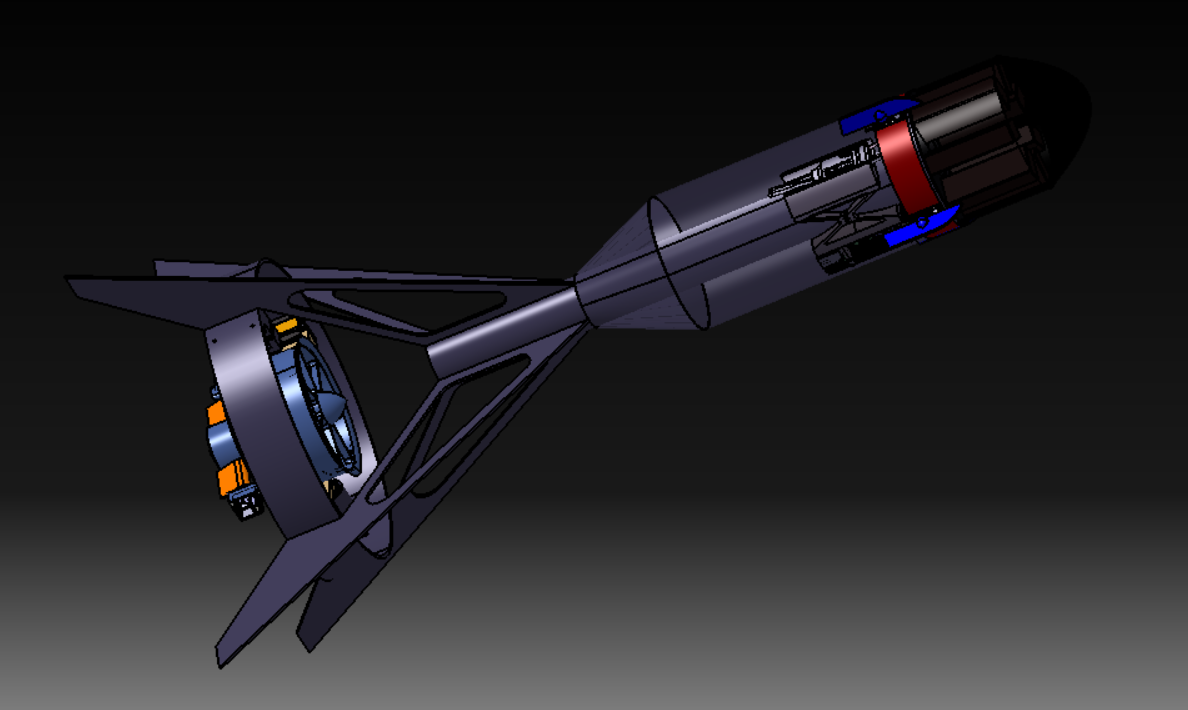
\includegraphics[width=\linewidth]{fig/design/1}
    \caption{Prototipo evolución al fuselaje de aluminio tubular, baterías en la nariz, sistema anti rolido en
    la parte superior, aviónica debajo de las baterías.}
    \label{fig:design/1}
\end{figure}

\begin{figure}[htb]
    \centering
    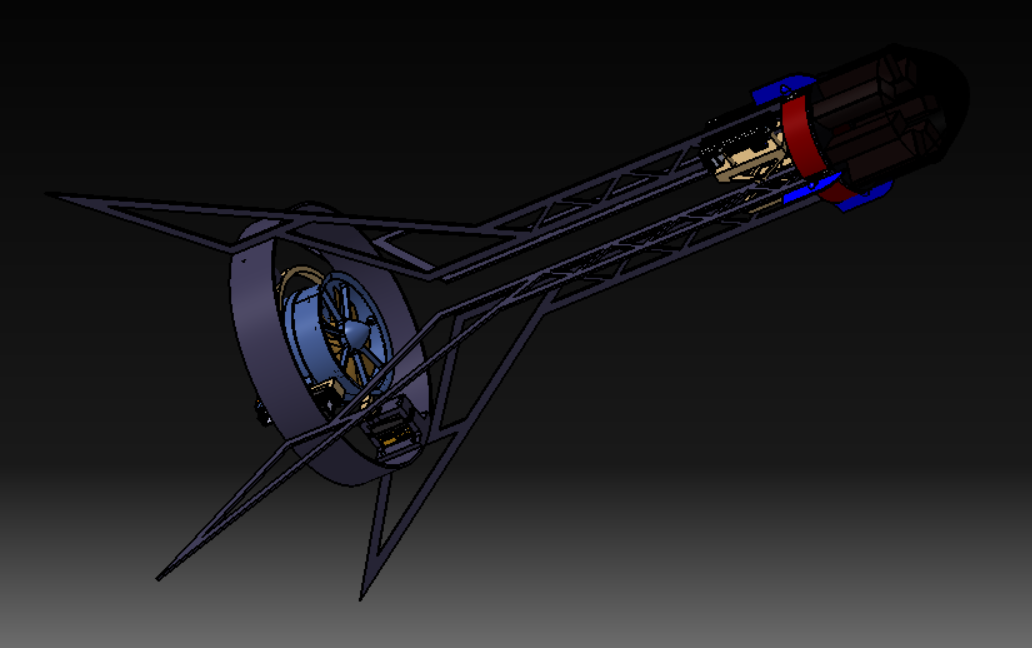
\includegraphics[width=\linewidth]{fig/design/2}
    \caption{Prototipo fuselaje reticulado de aluminio en forma de placas, baterías en la nariz, sistema anti
    rolido en la parte superior, aviónica debajo de las baterías.}
    \label{fig:design/2}
\end{figure}

\begin{figure}[htb]
    \centering
    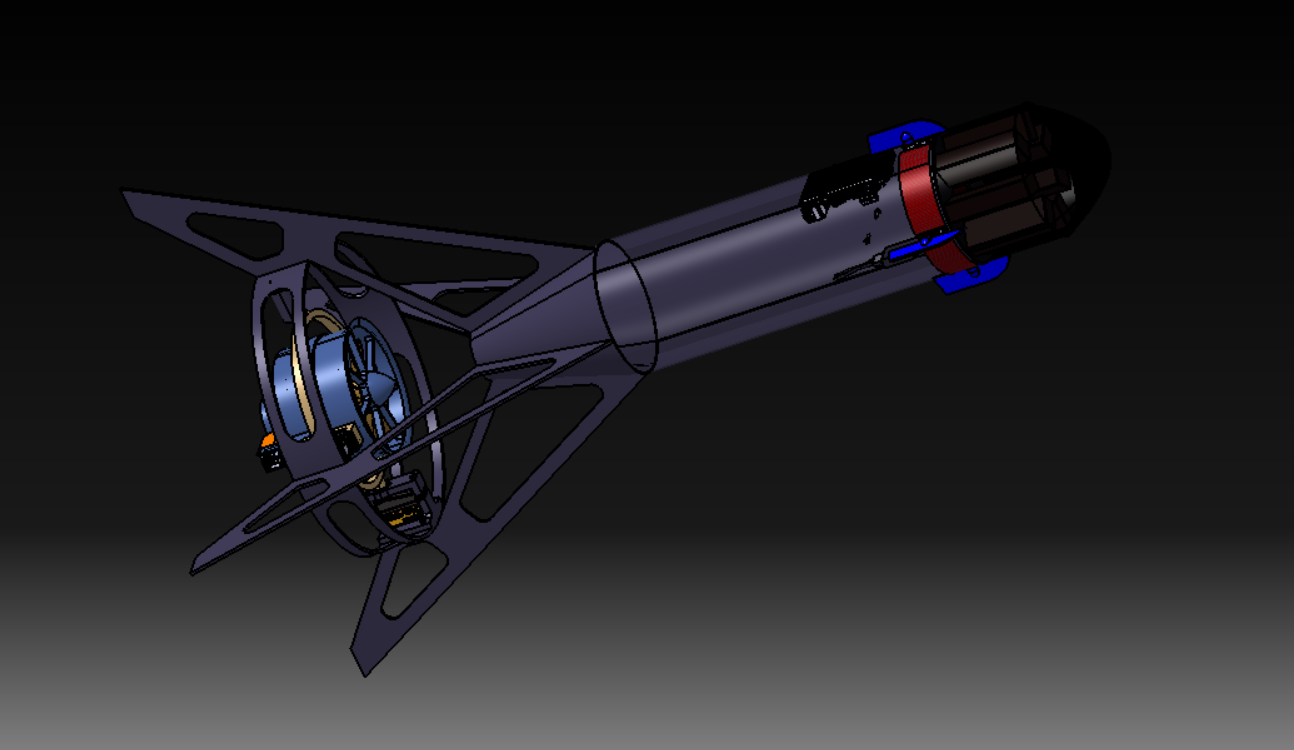
\includegraphics[width=\linewidth]{fig/design/3}
    \caption{Prototipo fuselaje reticulado de aluminio en forma de placas, baterías en la nariz, sistema anti
    rolido en la parte superior, aviónica debajo de las baterías.}
    \label{fig:design/3}
\end{figure}

\null\newpage
\clearpage
